\documentclass[a4paper,12pt]{article}

\usepackage[T2A]{fontenc}
\usepackage[utf8]{inputenc}
\usepackage[english,russian]{babel}
\usepackage[fontsize=14.0]{fontsize}
\usepackage[pdftex,unicode]{hyperref}
\usepackage{indentfirst}
\usepackage{amsmath}
\usepackage{amssymb}

\usepackage[left=30mm, top=25mm, right=15mm, bottom=25mm]{geometry}
\linespread{1.3}
\pagenumbering{arabic}

\usepackage[backend=biber, style=numeric, sorting=none]{biblatex}
\addbibresource{diploma.bib}

\usepackage{floatrow}
\usepackage{graphicx}
\graphicspath{ {pictures/} }

\begin{document}
	\begin{titlepage}
		\begin{center}
			
			
			
			{\small ФЕДЕРАЛЬНОЕ ГОСУДАРСТВЕННОЕ БЮДЖЕТНОЕ ОБРАЗОВАТЕЛЬНОЕ 
				УЧРЕЖДЕНИЕ ВЫСШЕГО ОБРАЗОВАНИЯ 
				
				<<МОСКОВСКИЙ ГОСУДАРСТВЕННЫЙ УНИВЕРСИТЕТ
				
				имени М.В. ЛОМОНОСОВА>>
				\ \\[1ex]
				ФИЗИЧЕСКИЙ ФАКУЛЬТЕТ МГУ }
			\ \\[0.8ex]
			Кафедра математического моделирования и информатики
			\ \\[0.8ex] 
			\hrule 
			
			\vspace{1cm}
			
			{\large КУРСОВАЯ РАБОТА}
			
			{\large\bf <<Нечеткая логика и ее практическое применение>> \\}
			\ \\[2ex]
			\begin{flushright}
				\begin{minipage}{0.42\textwidth}
					{\bf Выполнил}  \\ студент 204 группы \\ Павлов~Д.~М.
					\vspace{8mm}
					\vspace{1mm}
					{\small }
					\\[1ex]
					{\bf Научный руководитель} \\ к.ф.-м.н. Зубюк~А.~В.
					
					\vspace{40mm}
					
				\end{minipage}
			\end{flushright}
		\end{center}
		\hspace{3em}
		
		\vfill
		\vfill
		\begin{center}
			\vfill
			Москва\\
			2023
		\end{center}
		
	\end{titlepage}
	
	
	\newpage
	\setcounter{page}{2}
	
	\tableofcontents
	
	\newpage
	\setcounter{page}{3}
	\pagestyle{plain}
	\section*{Введение}
	В последние десятилетия наблюдается стремительное развитие нечеткой логики и смежных с ней дисциплин. Относительная простота математического аппарата и легкость разрабатываемых моделей привлекает все больше специалистов в эту область. По этой причине автор данной работы ставит для себя целью ознакомиться с основами нечеткой логики и исследовать простейший случай ее применения на практике.
	

	\section{Зачем нам нужна нечеткая логика?} 

	Часто на практике приходиться сталкивать с ситуацией, когда часть информации неизвестна полностью. Это может быть связано с погрешностью приборов, несовершенством модели или сложностью исследуемого процесса. В большинстве случаев эта неточность сводиться к двум пунктам:
	\begin{enumerate}
		\item недостаточно полное знание о предметной области в целом;
		\item недостаточная информация о конкретной ситуации.
	\end{enumerate}

	Располагая неполным знанием, мы не можем уверенно предсказать исход наших действий. Кроме того возможны ситуации, что даже когда мы располагаем достаточно полной теорией предметной области, эксперт может посчитать, что эффективно использовать не количественные, а качественные методы.  
	
	Одним из хорошо зарекомендовавших себя методов в условиях неопределенности является теория вероятностей. Однако и она сталкивается с определенными трудностями. Например, большой объем вычислений и проблема количественной оценки вероятности, выраженной лингвистически: «в большинстве случаев», «в редких случаях» и т.д. 
	Другим подходом к обработке неопределенной информации является предложенная в 60-х годах прошлого века американским математиком Лотфи Заде теория нечетких множеств (fuzzy set theory), представляющая собой формализм, предназначенный для формирования суждений о нечетких категориях и принадлежащих к ним объектах. Эта теория лежит в основе теории нечеткой логики (fuzzy logic) \cite{Zade}. Привлекательность нечеткой логики для проектировщиков экспертных систем состоит в ее близости к естественному человеческому языку. Таким терминам, как «быстрый», «медленный», чаще всего дается интерпретация на основе повседневного опыта и интуиции. Это упрощает процесс обработки информации, поскольку подобные суждения человека (эксперта) можно непосредственно преобразовать в выражения нечеткой логики.
	
	\section{Нечеткое множество}
	
	В классической теории множеств элемент либо принадлежит заданному множество, либо нет. Какая-либо неточность не допускаются при определении включения элемента. Элементы же нечетких множеств допускают некую неопределенность при описании их принадлежности заданному нечеткому множеству. Для количественного описания вводиться \textit{функция принадлежности} $\mu$, которая ставит в соответствие каждому элементу универсального множества U вещественное число из сегмента от 0 до 1, где 0 означает, что элемент однозначно не принадлежит множеству, а 1 — однозначно принадлежит:
	\[ \forall x \in U, \mu(x): U{\longrightarrow }Y, \]
	где  $Y=[0,1]$.
	
	\textit{Универсальное множество U} — множество всех элементов, для которых будет устанавливаться степень соответствия некоторому множеству. 
	
	\begin{figure}[h]
		\centering
		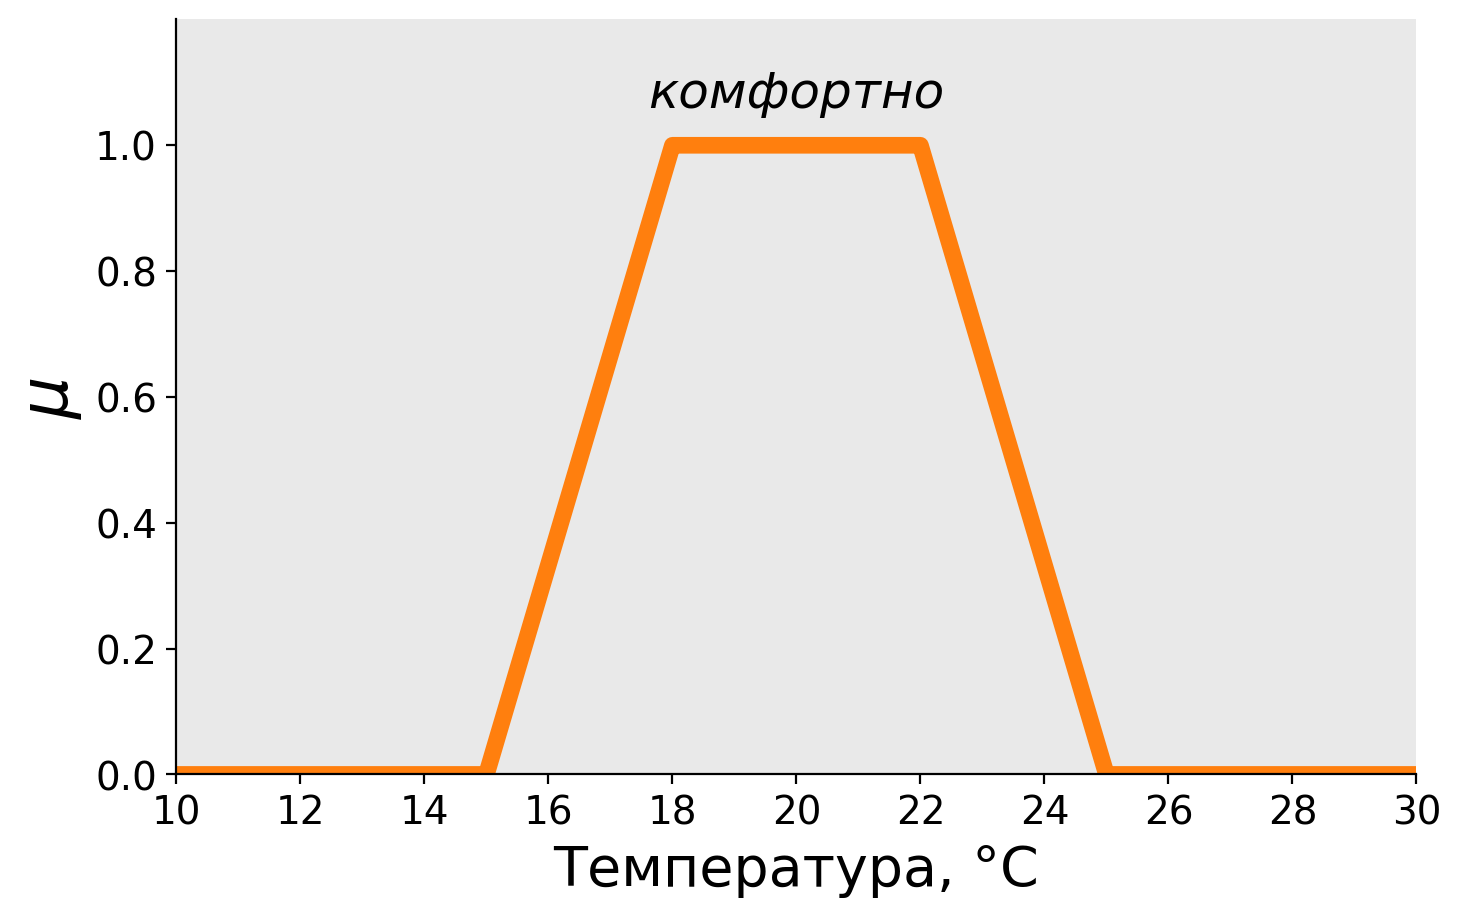
\includegraphics[width=0.5\textwidth]{Figure_1_1}
		\caption{График функции принадлежности нечеткого множества комфортной температуры}
		\label{fig:1_1}
	\end{figure}
	
	На рисунке~\ref{fig:1_1} видно, что температуры T~$\in$~[18, 20] являются однозначно некомфортными ($\mu=0$), T из [10, 15] и [25, 30] являются однозначно комфортными ($\mu=1$), а вот отношения для температур из [15, 18] и [22, 25] неопределенны однозначно. Они не являются некомфортными, но и не являются полностью комфортными, поэтому для их описания удобно использовать численное значение. Данные температуры как бы сразу принадлежат и не принадлежат нечеткому множеству комфортной температуры. Сам Заде сравнивал нечеткое множество с саквояжем, стенки которого являются "мягкими" \cite{Zade}.
	
	\section{Лингвистическая переменная}
	Кроме приведенного выше множества комфортной температуры на заданном универсальном множестве могут быть определены и другие нечеткие множества. Лингвистический термин, для которого определенные нечеткие множества могут рассматриваться как характеристики состояния этого термина, называется \textit{лингвистической переменной} $\chi$. Множество всех таких нечетких множеств называется \textit{терм-множеством} $T(\chi)$, а сами нечеткие множества — \textit{термами}. На рисунке~\ref{fig:1_2} температура является лингвистической переменной $\chi$, а терм-множество $T(\chi)=$\{холодно, комфортно, жарко\}.
	
	\begin{figure}[h]
		\centering
		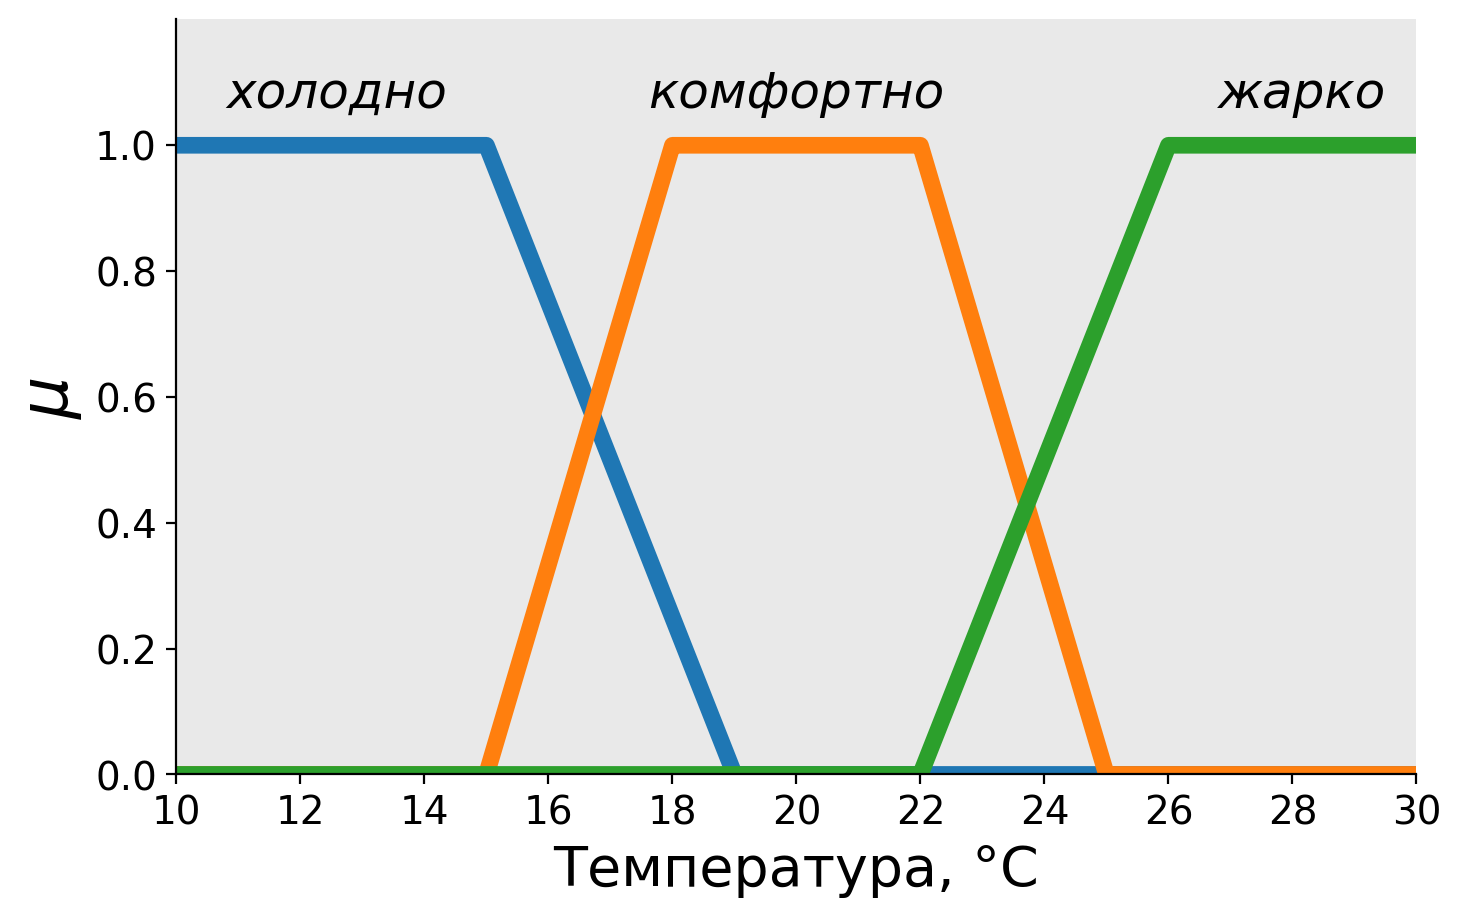
\includegraphics[width=0.5\textwidth]{Figure_1_2}
		\caption{График функции принадлежности нечеткого множества ``Комфортная температура''}
		\label{fig:1_2}
	\end{figure}

	Четкой переменной «17 $^\circ$C» будет соответствовать набор \{0.5, 0.67, 0\}, определяющий нечеткость в принадлежности этой переменной заданным термам.
	
	\section{Система нечеткого вывода}
	В целом вся система нечеткого вывода может быть представлена блок-схемой на рисунке~\ref{schm:1}:
	
	\begin{figure}[h]
		\centering
		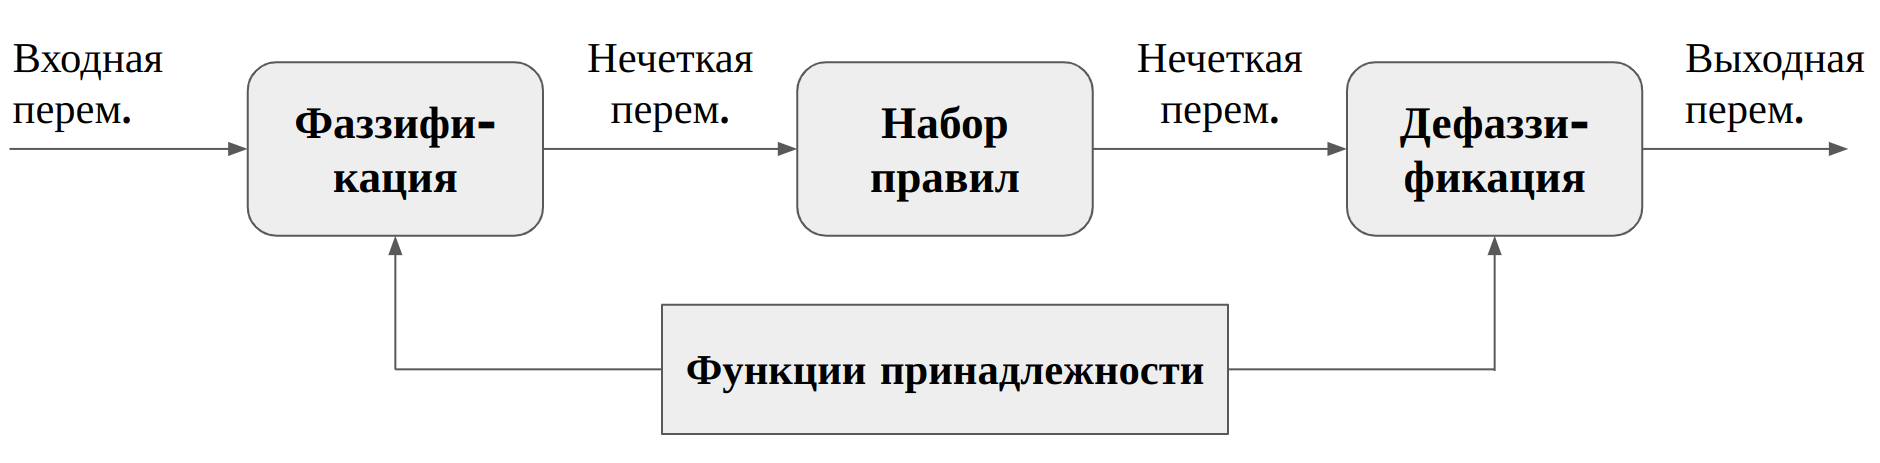
\includegraphics[width=1\textwidth]{scheme_1}
		\caption{Блок-схема системы нечеткого вывода}
		\label{schm:1}
	\end{figure}
	
	Существенным здесь является то, что поступающие обычные (четкие) переменные в процессе фаззификации \footnote{В английском языке используется слово \textit{fuzzy} — (в перев.) неясный неопределенный. Этим обоснованы слова «фаззификация» и «дефаззификация», т.е. процесс приведение четкой информации в нечеткую и наоборот.} становятся нечеткими, обрабатываются по правилам нечеткой логики и после очередного преобразования (дефаззификации) становятся снова однозначными. Фаззификация в большинстве случаев проводиться так же, как это было сделано выше для 17 $^\circ$C. В зависимости от поставленной задачи обработка и дефаззификация могут проводиться различными способами, ознакомиться с которыми подробнее можно в \cite{Dubya}.  
	
	\section{Используемые методы}
	
	В данной работе я использовал \textit{минимаксный} подход для обработки нечеткой информация. Данный подход весьма удобен, если набор правил определен в виде \textbf{ЕСЛИ} (...), \textbf{ТО} (...), с использованием логических операций \textbf{И}, \textbf{ИЛИ}, \textbf{НЕ}, и где аргументами выступают нечеткие переменные. В таком случае операция \textbf{И} заменяется на нахождение минимального значения, \textbf{ИЛИ} — максимального, \textbf{НЕ} заменяется разностью единицы и соответствующей нечеткой переменной.\\
	
	\underline{\textbf{Пример:}}\\
	\textbf{ЕСЛИ} ($P_1$ \textbf{И} \textbf{НЕ} $P_2$) \textbf{ИЛИ} $P_3$, \textbf{ТО} $B$.\\
	Что в минимаксном подходе соответствует формуле:
	\[B=max\{min\{P_1, 1-P_2\}, P_3\}\]
	
	Очевидно, что если $P_1, P_2, P_3 \in [0,1]$, то и $B \in [0,1]$.
	\\
	При известных функция принадлежности выходных переменных и при обработке, заданной выше образом, удобно проводить дефаззификацию с помощью метода "центра масс". Для каждого терма выходной лингвистической переменной (рисунок~\ref{fig:2_1}) с помощью минимаксного подхода вычисляется свой "вес"(значение~$B$). После чего область под каждым графиком "заполняется" до значения соответствующего "веса" (рисунок~\ref{fig:2_2}). 
	
	\begin{figure}[h]
		\centering
		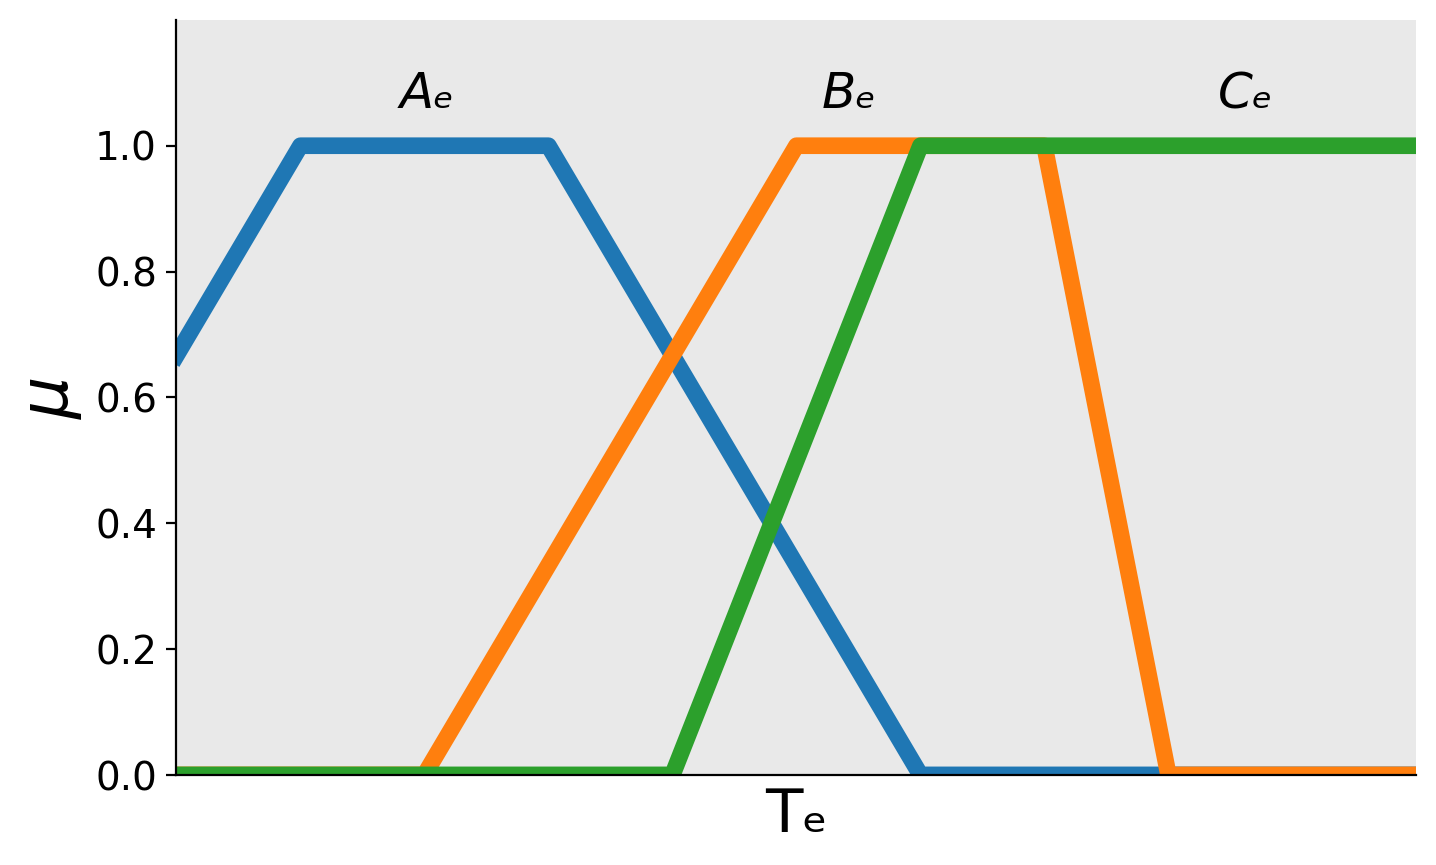
\includegraphics[width=0.5\textwidth]{Figure_2_1}
		\caption{Функции принадлежности}
		\label{fig:2_1}
	\end{figure}

	\begin{figure}[h]
		\centering
		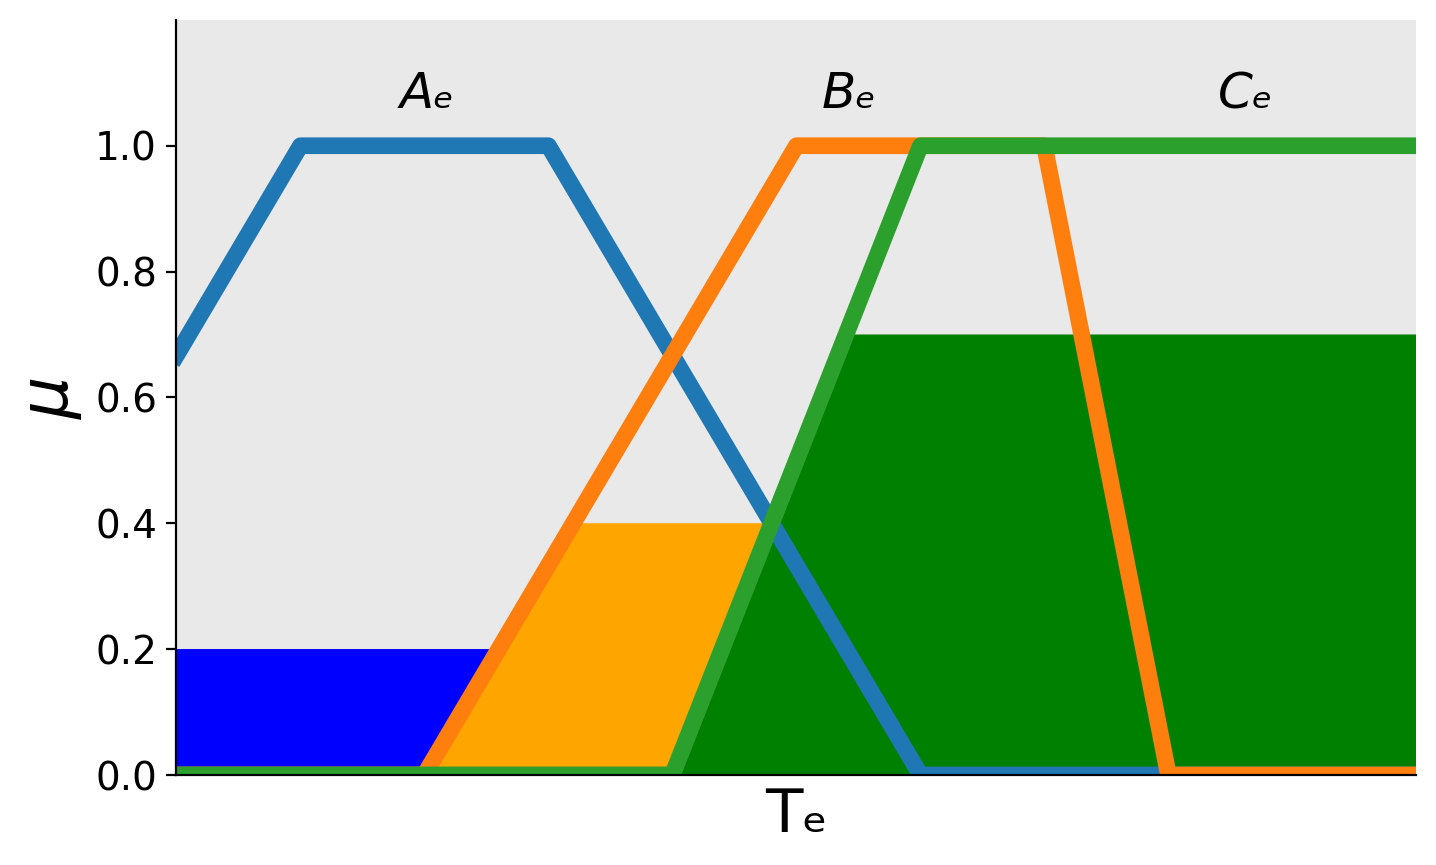
\includegraphics[width=0.5\textwidth]{Figure_2_2}
		\caption{Заполненные области}
		\label{fig:2_2}
	\end{figure}

	\begin{figure}[h]
		\centering
		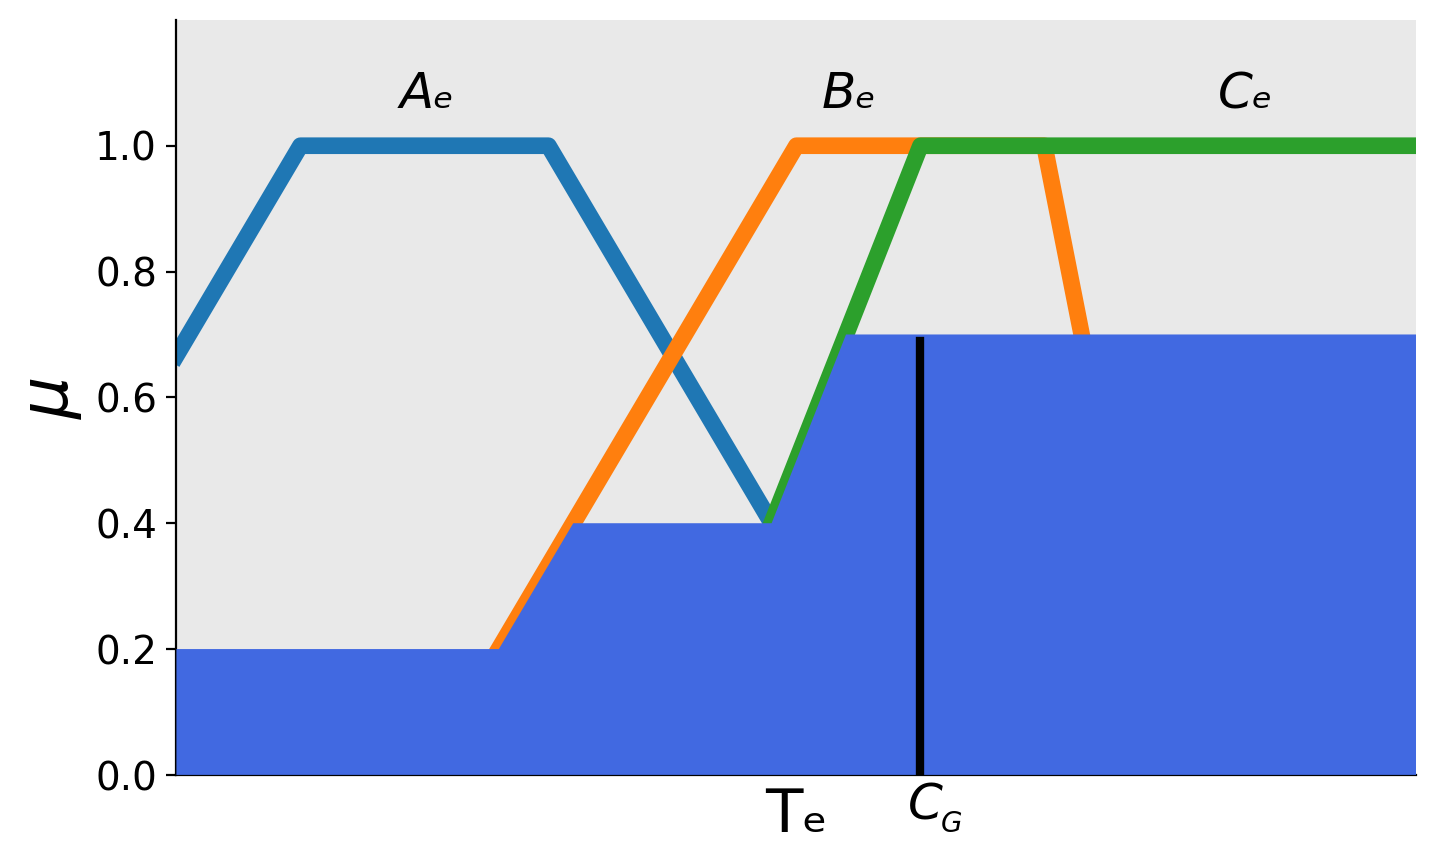
\includegraphics[width=0.5\textwidth]{Figure_2_3}
		\caption{Нахождения ``центра масс''}
		\label{fig:2_3}
	\end{figure}
	
	Далее, объединив эти области (рисунок~\ref{fig:2_3}), можно найти значение дефаззифицированной переменной по формуле:
	\[C_G=\cfrac{\displaystyle\sum_{U} x\mu(x)}{\displaystyle\sum_{U} \mu(x)}\]
	
	Геометрический смысл метода состоит в нахождении "центра масс" получившейся фигуры. Идею подхода легко понять, т.к. чем "тяжелее" фигура в некоторой области универсального множества, тем сильнее получившееся значение должно быть ближе к этой области.


	\section{Пример использования нечеткой логики}
	
	Рассмотрим практическое применение нечеткой логике, с помощью примера, который был смоделирован мною с использованием языка программирования Python.
	
	\underline{\textbf{Постановка задачи:}}\\
	Существует кулинарный продукт, массовое производство которого необходимо наладить. Рецепт продукта известен кондитеру, которого в подобных задачах принято называть \textit{экспертом}. Однако при описании рецепта возникает необходимость перевода лингвистических терминов, используемых кондитером (медленный огонь, пару чайных ложек и т. д.), в количественные переменные, с которыми могла бы работать машина. Пользуясь нечеткими множествами, эту проблема можно решить довольно легко. Опросив кулинара (т. е. получив экспертное мнение), можно установить соответствие между физическими величинами (мощностью, концентрацией, массой), поддающимися измерению, и степень соответствия этих величин заданным термам в представлении самого эксперта. Тем самым мы получим функции принадлежности для термов входных и выходных лингвистических переменных (Входные: рисунки~\ref{fig:3_1}~и~\ref{fig:3_2}, выходная: рисунок~\ref{fig:3_3}).
	
	\begin{figure}
		\begin{floatrow}[3]
			\ffigbox{\caption{}\label{fig:3_1}}
			{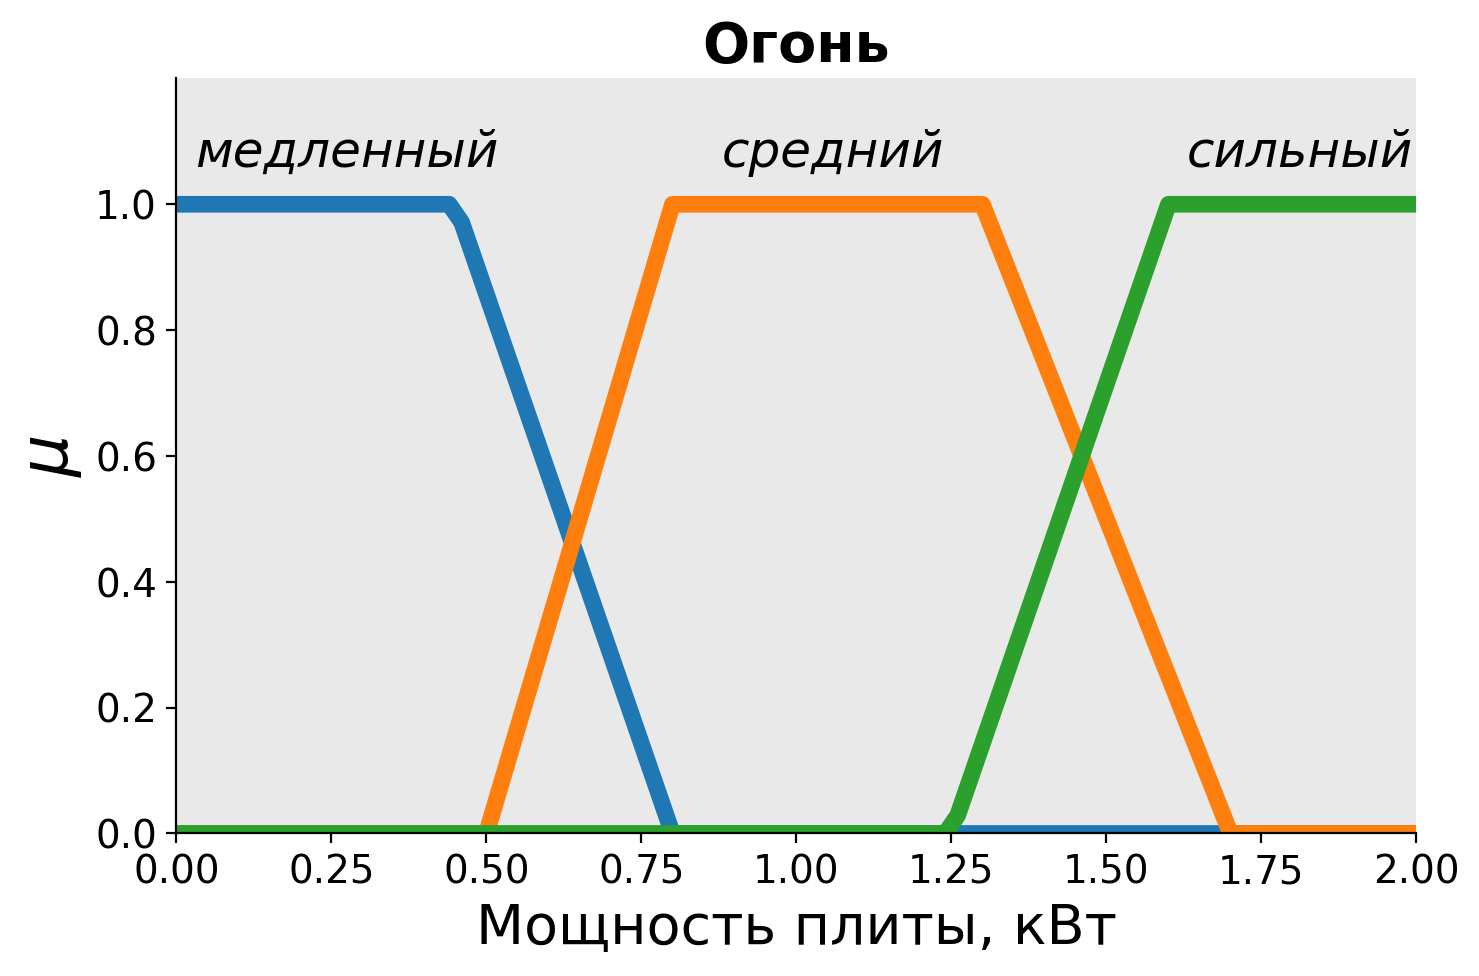
\includegraphics[width=0.3\textwidth]{Figure_3_1}}
			\ffigbox{\caption{}\label{fig:3_2}}
			{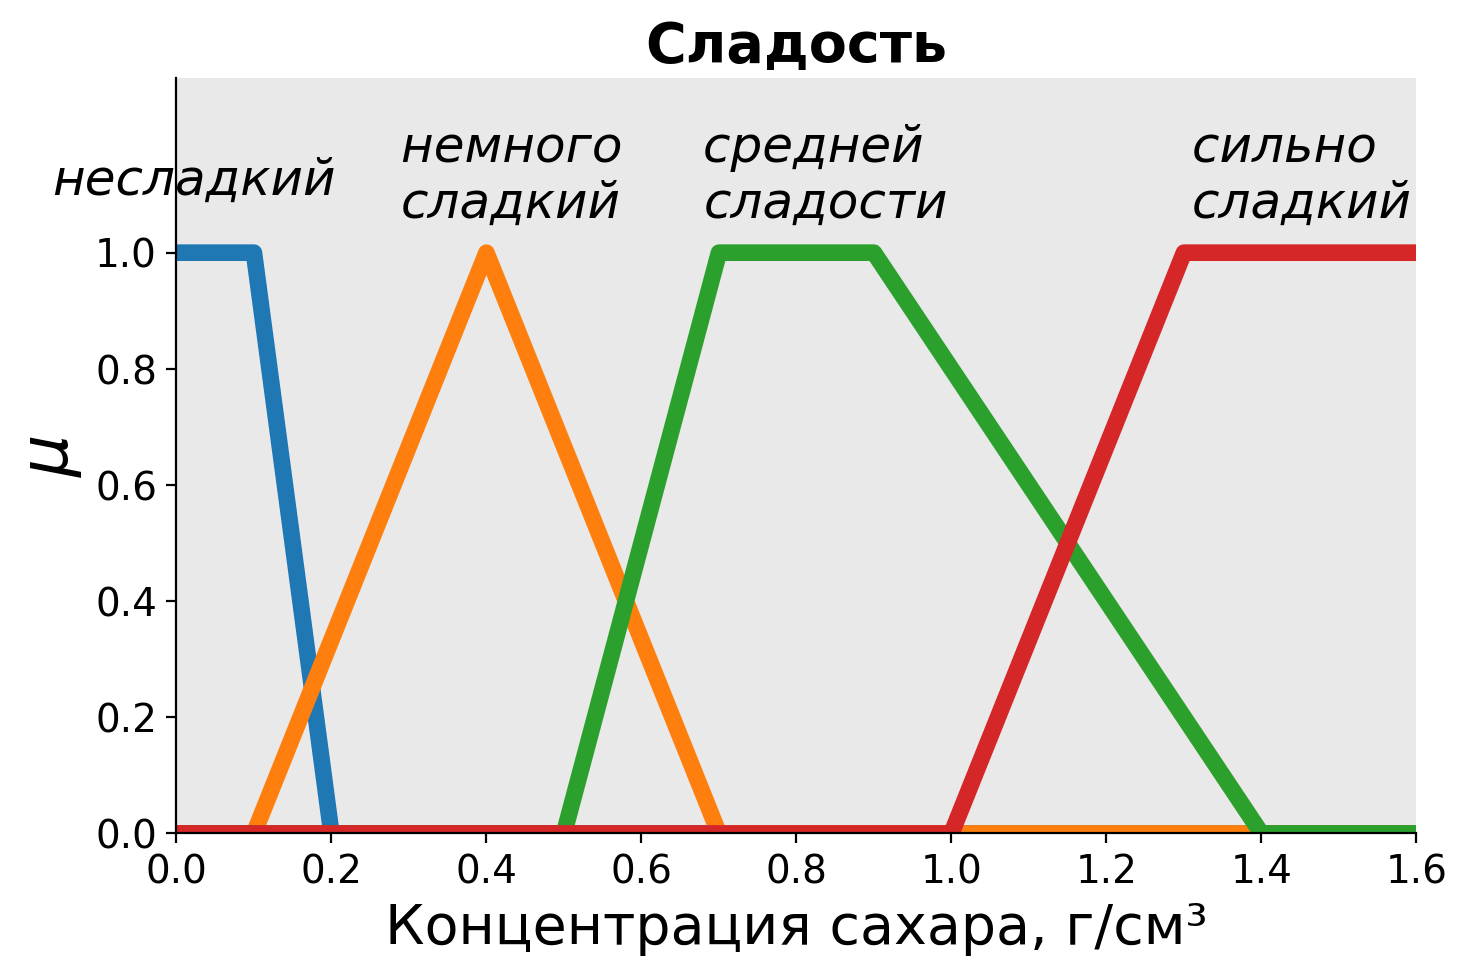
\includegraphics[width=0.3\textwidth]{Figure_3_2}}  
			\ffigbox{\caption{}\label{fig:3_3}}
			{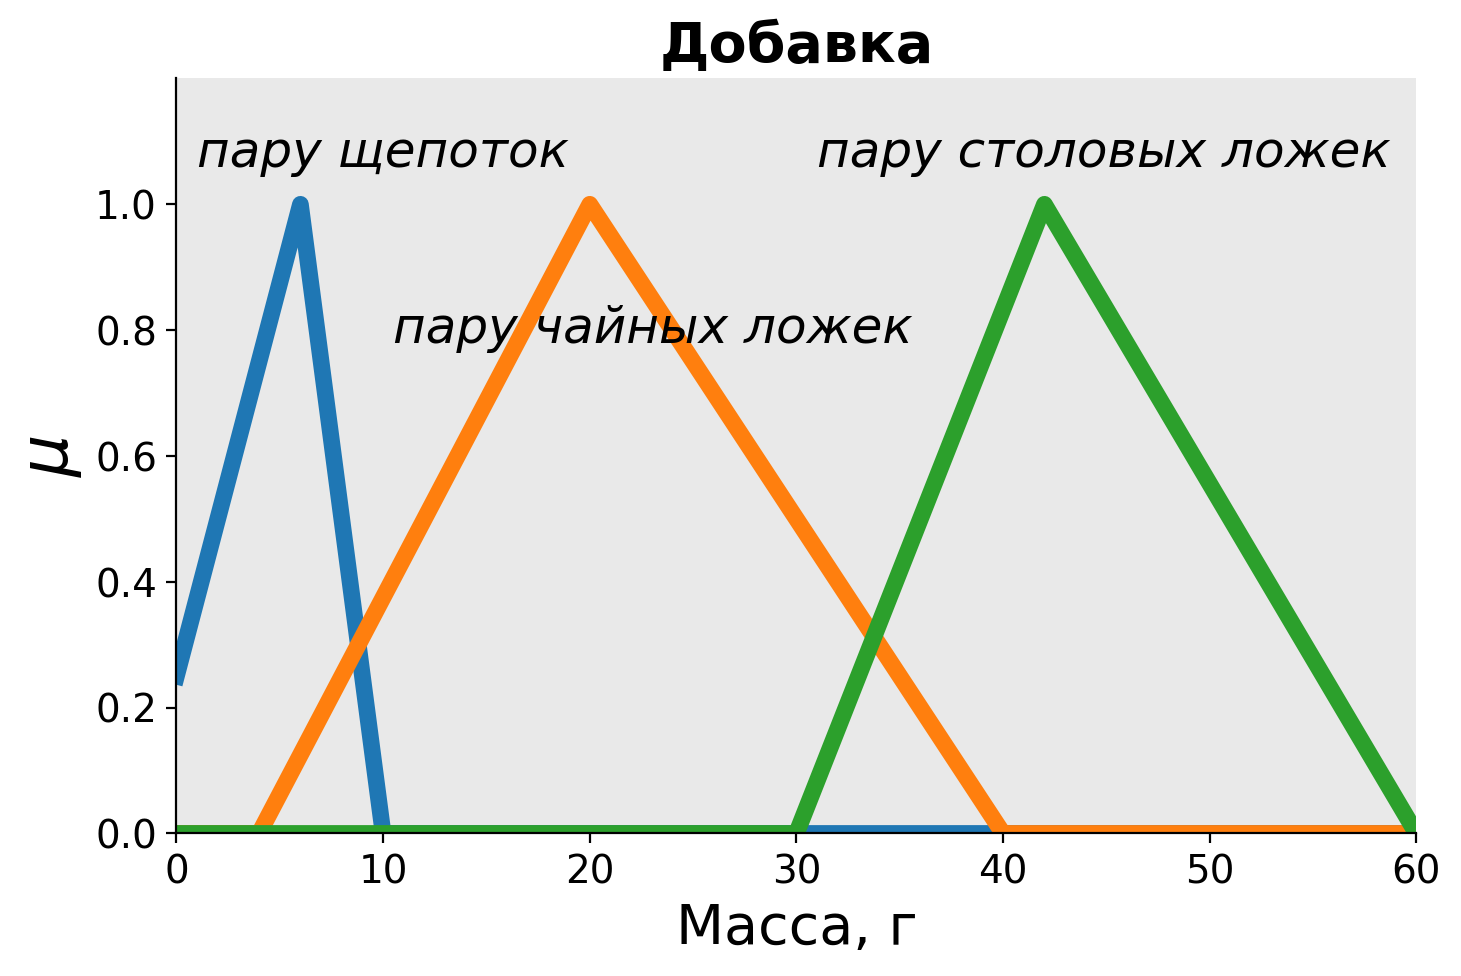
\includegraphics[width=0.3\textwidth]{Figure_3_3}}       
		\end{floatrow}
	\end{figure}
	Аналогичным образом можно перевести набор правил, используемых экспертом, в правила обработки, используя минимаксный подход.
	\\\\
	\underline{Набор правил эксперта:}
	
	\textbf{ЕСЛИ} (огонь \textit{медленный} \textbf{И} продукт \textit{немного сладкий})\\ \textbf{ИЛИ} ((\textit{огонь медленный} \textbf{ИЛИ} \textit{огонь сильный})\\ \textbf{И} продукт \textit{немного сладкий})\\ \textbf{ИЛИ} (огонь \textit{сильный} \textbf{И} продукт \textit{сильно сладкий}),\\ \textbf{ТО} добавить \textit{пару щепоток} ингредиента
	\\
	
	\textbf{ЕСЛИ} (огонь \textit{средний} \textbf{ИЛИ} (продукт \textit{средней\\ сладости} \textbf{ИЛИ} продукт \textit{немного сладкий}))\\ \textbf{ИЛИ} (огонь \textit{сильный} \textbf{И} продукт \textit{средней сладости})\\ \textbf{ИЛИ} (огонь \textit{медленный} \textbf{И} продукт \textit{сильно сладкий}),\\ \textbf{ТО} добавить \textit{пару чайных ложек} ингредиента
	\\
	
	\textbf{ЕСЛИ} (огонь \textit{медленный} \textbf{И} продукт \textit{сильно сладкий})\\ \textbf{ИЛИ} (огонь \textit{средний} \textbf{И} продукт \textit{средней сладости}),\\ \textbf{ТО} добавить \textit{пару столовых ложек} ингредиента
	\\
	
	Таким образом для каждого набора входных переменных определен алгоритм, дающий выходное (четкое) значение. В общем случае можно найти значение выходной переменной для любого элемента декартового произведения универсальных множеств входных переменных, что и было мною осуществлено. Т.к. в данном примере общее значение универсальных множеств $U$ (входных и выходных) равно трем, то можно представить результат моделирования графически (рисунок~\ref{fig:4_1}).
	
	\begin{figure}[h]
		\centering
		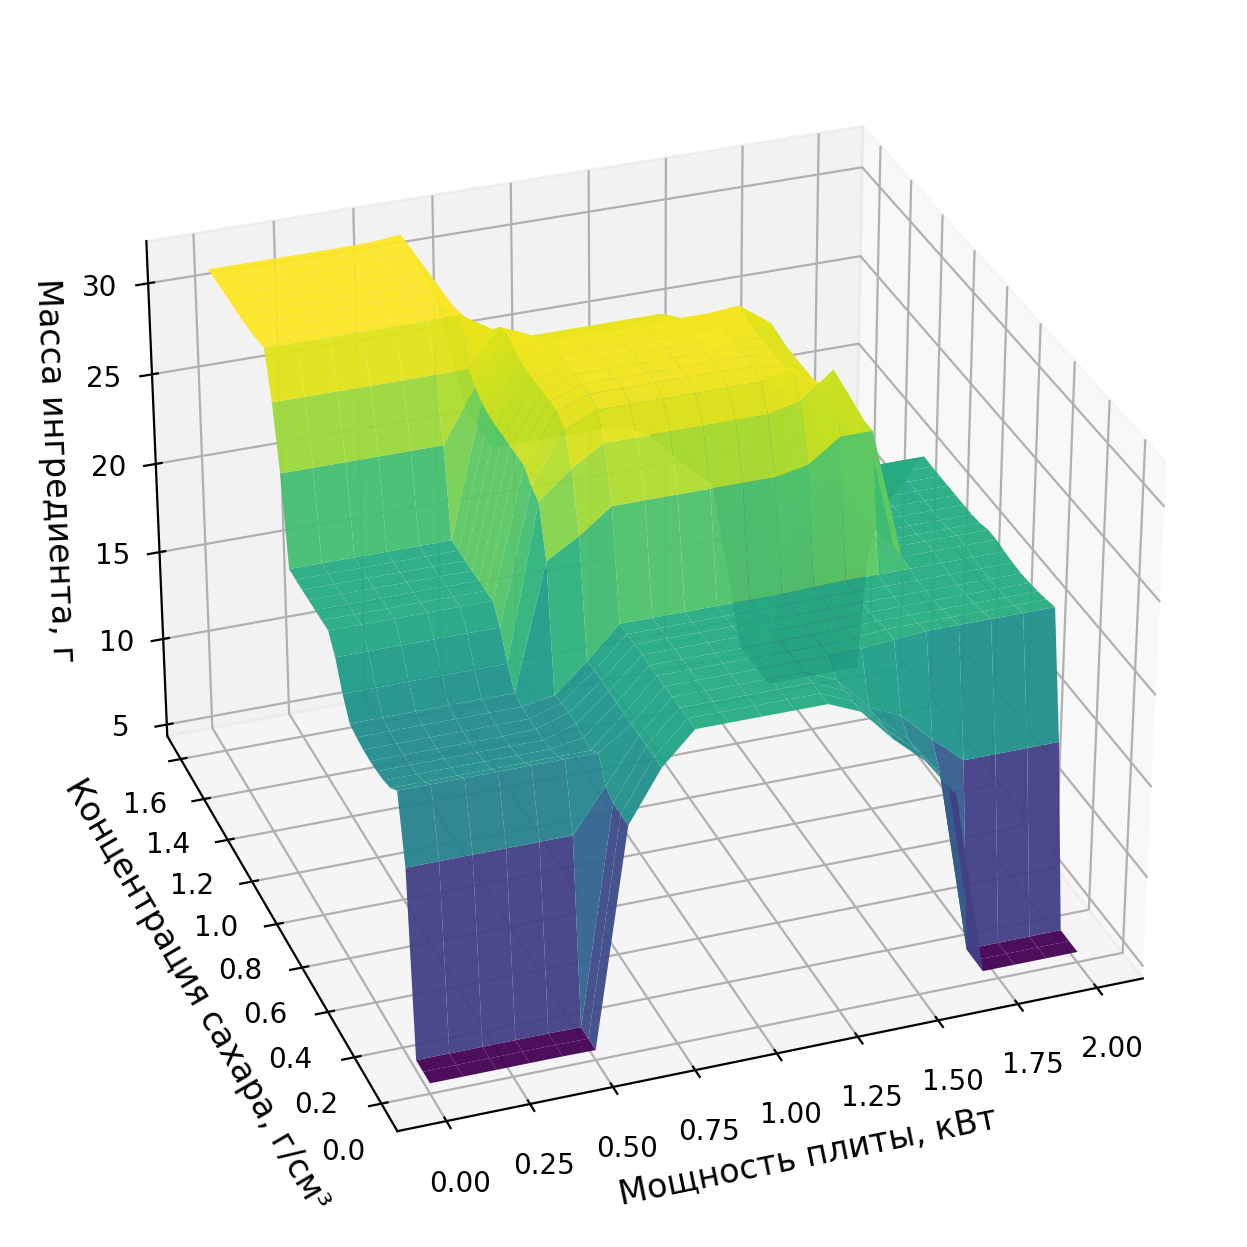
\includegraphics[width=0.8\textwidth]{Figure_4_1}
		\caption{График зависимости выходной переменной ``Масса ингредиента'' от входных переменных ``Мощность плиты'' и ``Концентрация сахара''}
		\label{fig:4_1}
	\end{figure}

	В некоторых случаях подобное графическое представление может помочь в понимании принципа работы. Подобные системы распространены, ведь лучше строить алгоритм по уже имеющимся правилам, полученным импирическим образом, чем строить сложную модель, пытаясь предвидеть поведение системы. Сама же зависимости может быть занесена в память машины, осуществляющей процесс контроля автоматического приготовления.
	
	
	\section{Выводы}
	
	В ходе проделанной работы мною были изучены основы нечеткой логики, исследована научная литература из соответствующей области, смоделировано применение нечетких множеств и нечеткой логики на практике для осуществления производственного процесса.
	
	Нечеткая логика прекрасно справляется с описанием нечеткой или неточной информации. Данное утверждение подтверждается не только рассмотренным мною примером, но и огромным количеством научных работ, которые публикуются учеными во всем мире.
	
	Нечеткая логика хорошо описывает многозначные лингвистические понятия. По этой причине она широко используется для моделирования человеческого мышления. Нечеткая логика используется в машинном обучение и нечетких нейронных сетях. 
	
	Простота и лаконичность разработки систем нечеткого логического вывода обуславливает их широкое применение как в коммерческой области (бытовые приборы, система «Умный дом», распознавание изображений и т.п.), так и в военной (беспилотные летательные аппараты, средства наведения ракет, управление боевыми вертолетами и т. п.).
	Многие современные задачи управления просто не могут быть решены классическими методами из-за очень большой сложности математических моделей, их описывающих. По этим причинам нечеткая логика уже стала неотъемлемой частью нашей жизни, пускай большинство людей этого и не замечает.
	
	\newpage
	\printbibliography

\end{document}